\documentclass[12pt]{article}

% sbc template
\usepackage{sbc-template}
\usepackage{graphicx,url}
\usepackage[utf8]{inputenc}

% equations
\usepackage{amsmath}
\usepackage{multicol}
\usepackage[version=4]{mhchem}
\usepackage{multicol}

% code snippets
\usepackage{graphicx}
\usepackage{listings}
\usepackage{xcolor}

% gro language definition
\definecolor{COLOR_COMMENTS}{RGB}{16, 97, 35}
\definecolor{COLOR_BACKGROUND}{RGB}{230, 230, 230}
\lstdefinelanguage{GROLANG}{
  morekeywords    =   {include,program,rate,ecoli},
  sensitive       =   false,
  morecomment     =   [l]{//},
  morestring      =   [b]",
}
\lstdefinestyle{GROSRC}
{
  language          =   GROLANG,
  basicstyle        =   \footnotesize\ttfamily,
  keywordstyle      =   \color{black}\bfseries,
  extendedchars     =   true,
  commentstyle      =   \color{COLOR_COMMENTS},
  backgroundcolor   =   \color{COLOR_BACKGROUND},
  frame             =   single,
  caption           =   Dummy gro file.,
  tabsize           =   4,
  breaklines        =   true,
  showstringspaces  =   false,
}

% parsed.intermediate style definition
\lstdefinestyle{INTERMEDIATE}{
  basicstyle        =   \footnotesize\ttfamily,
  backgroundcolor   =   \color{COLOR_BACKGROUND},
  otherkeywords     =   {compartment, var, const, in},
  keywordstyle      =   \color{black}\bfseries,
  frame             =   single,
  tabsize           =   4,
  caption           =   Compiled dummy.,
  breaklines        =   true,
  showstringspaces  =   false,
}

% begin paper
\sloppy
\title{Albi:\\ A gro compiler to the SBML standard}
\author{Alek Frohlich\inst{1}, Gustavo Biage\inst{1}}
\address{Departamento de Informatica e Estatística – Universidade Federal de Santa Catarina \\
Florianopolis – SC – Brazil
  \email{\{alek.frohlich,gustavo.c.biage\}@grad.ufsc.br}
}
\begin{document}
\maketitle
\begin{abstract}


    The growth of research areas such as synthetic biology and systems biology leads to an increased tendency to develop larger mathematical models for describing complex biological behavior. In order to enable natural flow of development of those models, scientists must have access to tools which increase the level of abstraction and enable the reuse of biological components. The present work tackles those two problems by integrating the existing programming language gro with the SBML standard for model interchangeability and ease of model design.


\end{abstract}
\section{Introduction}


    Even though a Systems Biology Markup Language API (LibSBML) has already been developed \cite{Bornstein2008}, it only ought to be useful in cases where a new model is to be developed. In cases where there is a preexisting model, the availability of an SBML library does not help much since the previous model would have to be entirely rewritten to fit the API. Instead, the present work proposes an integration scheme that uses a language parser to generate SBML documents from previously built gro models. Gro is a language for programming, modeling, specifying and simulating the behavior of cells in growing microcolonies of microorganisms \cite{Jang2012}. The parser has been built upon it considering gro has many interesting syntactical constructs such as rate statements\footnote{Here, and all throughout this paper we shall refer to expressions guarded by gro's rate function as rate statements.}, program definitions and bacterial instantiation which can be expressed, respectively, as reactions, local name spaces and compartments in SBML documents.
    
    In regards to language support, gro is still tightly coupled with it's original simulator. Although the simulator has recently undergone big improvements in the sense that simulations behave more realistically \cite{Gutirrez2017}, it doesn't change the fact that using it is the only available way to validate gro models. This hinders the reproducibility of experiments built with the language. SBML models, on the other hand, are supported by more than 100 software systems \cite{Hucka2007}, making them more likely to be verified and reused.
    
    If gro code were translated into SBML, the resulting document could then be further preserved as an entry in BioModels. BioModels is a database of curated SBML and CellML models intended to provide researchers with models related to a particular disease, biological process or molecular complex \cite{LeNovere2006}. Having a model curated is an even stronger guarantee of trustworthiness since the process is done manually for each model: Newly submitted models go through a series of syntactical analysis to confirm that they are valid and well formatted; The model is then numerically verified against the results claimed by the authoring paper; Finally, the validated model gets manually annotated and cross-linked to facilitate later search for it \cite{LeNovere2006}.
    
    The rest of the paper is structured as follows: In Sect. 2, we introduce the language parser and explain the process of converting gro files to SBML models from start to finish; In Sect. 3, we demonstrate a possible use case for the proposed SBML integration scheme through simulating an SBML model generated from gro source code; In Sect. 4, we summarize what has been done and compare it with goals laid out at the start; In Sect. 5 we conclude by presenting possible extensions of the current work.
    

\section{Architecture}

    
    The compilation process is divided in three steps: First, the code is validated, that is, it's checked against syntax errors such as missing semicolon in rate statements and semantic error such as using undeclared variables; Then the code gets compiled to Antimony, a modular model definition language \cite{Smith2009}; This format guides Tellurium in building the final SBML document. As we'll see in the following subsections, Tellurium makes use of the aforementioned libSBML API for code generation purposes.


\subsection{The parser}
    
    The language parser was implemented using Flex, Bison and C. It currently recognizes only a subset of gro's syntax. Valid programs are constituted by global variable declarations, program definitions and E. coli instantiations. Parameters, messages and guarded statements are also recognized as valid syntax, however no semantic value is assigned to them given that control statements and user interaction do not make sense in the context of an SBML model. Below is an example of gro code containing the syntactical constructs just described.

    \begin{lstlisting}[style=GROSRC, caption=Example gro code.]
 include gro

 program prog() := {
     E := 25;
     F := 75 + E;
     K := 2 + F + E;
     rate(K) : { E := E + 1, F := F - 1 };
 };

 program dupl(X) := {
     E := 25 + X;
     F := 75 + E;
     K := 2 + F + E;
     rate(K*40) : { E := E + 1, F := F - 1 };
 };

 ecoli([], program prog() + dupl(10));
 ecoli([], program prog());
\end{lstlisting}
    
    Compiling this file gives the Antimony model that Tellurium in conjunction with libAntimony use to interact with libSBML. As we can see, the compiler properly handled arithmetic expressions and parameter passing. It did so to enable the use of gro program as a modelling tool for expressing parameterizable SBML models. The compiler also renamed symbols declared inside program definitions to avoid name space clashes between multiple programs instantiated in the same compartment. If this renaming hadn't been done, there wouldn't be a way to differentiate the symbol E, whose name space is limited to reactions inside of prog, from the symbol E which was declared inside of dupl.
    
    \input{example_compiled.tex}
    
\subsection{The Tellurium framework}

    Tellurium is a Python-based modeling environment for systems and synthetic biology \cite{Choi2018}. It aggregates multiple preexisting libraries such as libSBML, libAntimony and libSBOL to provide the modelling community access to an integrated modelling environment. Tellurium is organized in three functional pillars: Standards support, modelling support and utilities.


\section{Case study: The Repressilator}


    The goal of this experiment was to illustrate the proposed SBML integration scheme. It was conducted as follows: We first simulated the gro model for a well-known biological device, the Repressilator, in gro's built-in simulator; We then compiled the source code down to SBML following the steps shown in Sect. 2; Finally we simulated the compiled gro code, an SBML document, in COPASI. Finally, the COPASI simulation was compared against an Octave one for the original model. Both yielded the same result, indicating that the compiled model was the same as the original one.


\subsection{Mathematical Model}

    \begin{figure}[h]
        \centering
        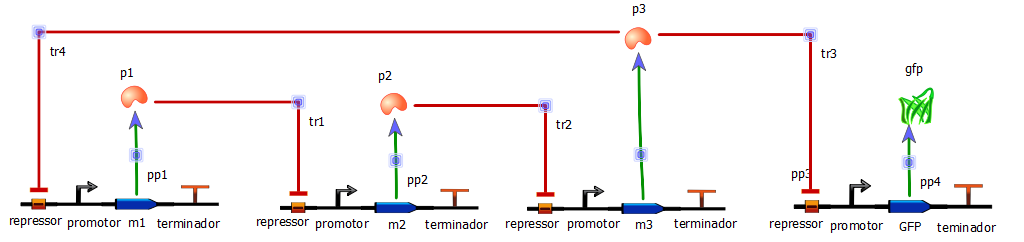
\includegraphics[scale = 0.7]{repressilator_model.png}
        \caption{Repressilator's genetic regulatory network.}
        \label{fig:repressilator_model}
    \end{figure}
    
    The Repressilator is a genetic regulatory network constituted by stitching together promoter-repressor pairs. It was first conceptualized by \cite{Elowitz2000}, who used the genes LacI and letR from E. coli and cI from phage lambda to build a three-repressor scheme. As illustrated in Figure~\ref{fig:repressilator_model}, the Repressilator works based on the fact that each gene expresses a protein which represses the next gene in the loop, meaning that a constituent gene in high concentration represses itself indirectly, leading to oscillatory behavior. In the original experiment, there was another biological component involved: the reporter, a green fluorescent protein (GFP) producing gene. It was used to visualize the network's oscillation.
    
    \begin{equation}
    \begin{aligned}[c]
        \frac{dm_{1}(t)}{dt} & = \alpha_{0} + \frac{\alpha}{1 + p_{3}(t)^{n}} - m_{1}(t) & \\
        \frac{dm_{2}(t)}{dt} & = \alpha_{0} + \frac{\alpha}{1 + p_{1}(t)^{n}} - m_{2}(t) & \\
        \frac{dm_{3}(t)}{dt} & = \alpha_{0} + \frac{\alpha}{1 + p_{2}(t)^{n}} - m_{3}(t) &
    \end{aligned}
    \begin{aligned}[c]
        \frac{dp_{1}(t)}{dt} & = \beta \cdot m_{1}(t) - \beta \cdot p_{1}(t) \\
        \frac{dp_{2}(t)}{dt} & = \beta \cdot m_{2}(t) - \beta \cdot p_{2}(t) \\
        \frac{dp_{3}(t)}{dt} & = \beta \cdot m_{3}(t) - \beta \cdot p_{3}(t)
    \end{aligned}
    \end{equation}

    As shown in \cite{Elowitz2000}, the high-level model from Figure~\ref{fig:repressilator_model} could also be presented as the above system of Ordinary Differential Equations (ODE)\footnote{The names given for the components of the Repressilator at (1) shall continue to be used as is for the rest of this section.}. With that system of equations, we then built the corresponding gro model. The process was simple as we just separated the reactions from the equations, meaning, for example, that $\alpha_{0}$ from the left equations became the open reaction:
    
    \begin{equation}
    \ce{ ->[\alpha_{0}] m_{1} + m_{2} + m_{3}}
    \end{equation}
    
    By repeating this process for each ODE, we ended up with a total of 7 reactions. As gro does not support reversible reactions directly through it's \textit{rate} function, each reversible one was split onto two new reactions: One for the forward part and another for the reverse. On doing so, the final gro model packed a total of 13 rate statements, all of whom can be observed below.
    
    \begin{lstlisting}[style=GROSRC]
 rate(alfa0) : { m1 := m1 + 1, m2 := m2 + 1, m3 := m3 + 1 };
 rate(alfa / (1 + p3^n)) : {m1 := m1 + 1};
 rate(m1) : {m1 := m1 - 1};
 rate(alfa / (1 + p1^n)) : {m2 := m2 + 1};
 rate(m2) : {m2 := m2 - 1};
 rate(alfa / (1 + p2^n)) : {m3 := m3 + 1};
 rate(m3) : {m3 := m3 - 1};
 rate(beta*m1) : {p1 := p1 + 1};
 rate(beta*p1) : {p1 := p1 - 1};
 rate(beta*m2) : {p2 := p2 + 1};
 rate(beta*p2) : {p2 := p2 - 1};
 rate(beta*m3) : {p3 := p3 + 1};
 rate(beta*p3) : {p3 := p3 - 1};
\end{lstlisting}

\subsection{Gro}
    
    Gro simulates multiple different aspects of the bacterial colony, including growth, division and contact forces between cells \cite{Jang2012}. Although that makes for a realistic multicellular simulator, it doesn't carry weight in single cell simulation such as the ones we did for the Repressilator shown in the last section. In it's case, the uniquely relevant aspect of it's simulation was how gro evaluated rate statements. As is indicated by \cite{Hoops2006}, at each simulation step, each guard is evaluated. If it evaluates to true, then the corresponding block is executed, meaning, in our case, that a reaction occurred.
    
    To model stochastic events, gro provides the \textit{rate} (\textit{r}) function that evaluates to true under the probability of r*dt, where the dt is the step size of the simulation. Simulation parameters in the likes of dt can be set by using the \textit{set} (\textit{key}, \textit{value}) function. Gro makes further use of the \textit{rate} function to approximate the Master Equation with Euler integration. 
    
    \begin{figure}[ht]
    \centering
    \minipage{0.33\textwidth}
      \includegraphics[width=\linewidth]{img1.png}
    \endminipage\hfill
    \minipage{0.33\textwidth}
      \includegraphics[width=\linewidth]{img2.png}
    \endminipage\hfill
    \minipage{0.33\textwidth}%
      \includegraphics[width=\linewidth]{img3.png}
    \endminipage
    \caption{Multiple simulations of the Repressilator gro model. From left to right: p1, p2, p3. Black lines are used to indicate an average simulation, whilst the various grey lines are used to indicate the concentration of the respective protein at each individual simulation.}
    \label{fig:tons_of_simulations}
    \end{figure}

   In Figure~\ref{fig:tons_of_simulations}, we see the results of simulating the Repressilator model within gro itself. Simulation parameters taken from \cite{ingalls2013mathematical}: $\alpha_{0} = 0.03$ (molecules per $cell \cdot min^{-1}$), $\alpha = 298.2$ (molecules per $cell \cdot min^{-1}$), $\beta = 0.2$ ($min^{-1}$), $n = 2$ and $\delta t = 0.0001$. The average simulation containing all of $p_{1}, p_{2}, p_{3}, m_{1}, m_{2}, m_{3}$ and illustrated by Figure~\ref{fig:repressilator_average} shows that the original period and amplitude varied during the course of time, probably due to stochastic fluctuations. From a naive perspective the model maintained it's oscillatory behavior. Delving deeper, we are able to conclude from Figure~\ref{fig:biffurcation} that, that the initial values picked for the simulations could be tuned to increase the robustness of the outcome under stochastic simulations.

    \begin{figure}[ht]
    \centering
    \minipage{0.5\textwidth}
      \includegraphics[width=\linewidth]{all_med_thick.png}
      \caption{Average of the protein's concentrations over multiple simulations.}
      \label{fig:repressilator_average}
    \endminipage\hfill
    \minipage{0.5\textwidth}
      \includegraphics[width=\linewidth]{biffurcation_a_b_2.png}
      \caption{Bifurcation graph for $\alpha$ and $\beta$.}
      \label{fig:biffurcation}
    \endminipage\hfill
    \end{figure}

\subsection{COPASI}
    
    COPASI is a software package for simulating chemical reactions. We chose to simulate the resulting SBML document on it because of the variety of simulation methods that it supports. Ranging all the way from deterministic methods such as LSODA \cite{Petzold1983} to stochastic ones like Gillespie’s algorithm \cite{Gillespie1976}. Unfortunately, gro does not implement Gillespie’s algorithm\footnote{Gro concurrently simulates growth, geometry, and signal dynamics. Meaning that any other resource-intensive simulation methods would be impractical due to performance reasons.}, thus we compared COPASI's output with that in \cite{Goeldner2019}, whom implement the same starting conditions as \cite{ingalls2013mathematical}. The simulations are shown in Figure~\ref{fig:repressilator_comparison}.
    
    \begin{figure}[ht]
    \centering
    \minipage{0.5\textwidth}
      \includegraphics[width=\linewidth]{octave_plot_thick.png}
    \endminipage\hfill
    \minipage{0.5\textwidth}
      \includegraphics[width=\linewidth]{SBML_copasi_LSODA.png}
    \endminipage\hfill
    \label{fig:repressilator_comparison}
    \caption{Comparison between the Octave model and compiled gro model for the Repressilator. The simulation was done using the same parameters as Figure~\ref{fig:repressilator_average}.}
    \end{figure}
    
    As per simple analysis of both graphs we can conclude that the behavior of both models was indeed similar. In order to prove that both mathematical models are identical, however, we need to compare the underlying systems of equations. To accomplish this, we explore the fact that COPASI infers math equations from the SBML model given to it. Hence, by looking at the equations bellow and comparing them to (1), we can conclude that the gro model from Listing 3 is the same as the Octave one.
    
    \begin{equation*}
    \begin{split}
        \frac{d([ECOLI0\_prog\_m1]*V_{ECOLI0})}{dt} & = +V_{ECOLI0}*(\frac{alfa + [ECOLI\_prog\_p3]^n}{V\_{ECOLI0}}) \\ & +V_{ECOLI0}*(\frac{alfa0}{V_{ECOLI0}})
        \\ & -V_{ECOLI0}*(\frac{[ECOLI0\_prog\_m1]}{V_{ECOLI0}})
    \end{split}
    \end{equation*}
    \begin{equation*}
    \begin{split}
        \frac{d([ECOLI0\_prog\_m2]*V_{ECOLI0})}{dt} & = +V_{ECOLI0}*(\frac{alfa + [ECOLI\_prog\_p1]^n}{V\_{ECOLI0}}) \\ & +V_{ECOLI0}*(\frac{alfa0}{V_{ECOLI0}})
        \\ & -V_{ECOLI0}*(\frac{[ECOLI0\_prog\_m2]}{V_{ECOLI0}})
    \end{split}
    \end{equation*}
    \begin{equation*}
    \begin{split}
        \frac{d([ECOLI0\_prog\_m3]*V_{ECOLI0})}{dt} & = +V_{ECOLI0}*(\frac{alfa + [ECOLI\_prog\_p2]^n}{V_{ECOLI0}})
        \\ & +V_{ECOLI0}*(\frac{alfa0}{V_{ECOLI0}})
        \\ & -V_{ECOLI0}*(\frac{[ECOLI0_prog_m1]}{V_{ECOLI0}})
    \end{split}
    \end{equation*}
    \begin{equation*}
    \begin{split}
        \frac{d([ECOLI0\_prog\_p1]*V_{ECOLI0})}{dt} & = -V_{ECOLI0}*(\frac{beta*[ECOLI\_prog\_p1]^n}{V_{ECOLI0}}) 
        \\ & +V_{ECOLI0}*(\frac{beta*[ECOLI\_prog\_m1]^n}{V_{ECOLI0}})
    \end{split}
    \end{equation*}
    \begin{equation*}
    \begin{split}
        \frac{d([ECOLI0\_prog\_p2]*V_{ECOLI0})}{dt} & = -V_{ECOLI0}*(\frac{beta*[ECOLI\_prog\_p2]^n}{V_{ECOLI0}}) 
        \\ & +V_{ECOLI0}*(\frac{beta*[ECOLI\_prog\_m2]^n}{V_{ECOLI0}})
    \end{split}
    \end{equation*}
    \begin{equation*}
    \begin{split}
        \frac{d([ECOLI0\_prog\_p3]*V_{ECOLI0})}{dt} & = -V_{ECOLI0}*(\frac{beta*[ECOLI\_prog\_p3]^n}{V_{ECOLI0}}) 
        \\ & +V_{ECOLI0}*(\frac{beta*[ECOLI\_prog\_m3]^n}{V_{ECOLI0}})
    \end{split}
    \end{equation*}


\section{Conclusion \& Future works}
    
    
    We have presented an SBML integration scheme for the gro language with the intent of facilitating the development of new SBML models and recovering previously built gro models, as was done in Sect. 3, with the Repressilator. The identical models provided there demonstrate the effectiveness of our proposed scheme. For it to be abragente, however, the language parser should be able to handle all possible gro programs. That's not currently the case as signalling and structures have not yet been implemented and could serve as practical extension of the current work.


% references
\bibliographystyle{sbc}
\bibliography{sbc-template}
\end{document}
